%!TEX root = ../research_proposal.tex


Field failures are challenging to reproduce because
the data provided by the end users is often scarce. A survey
conducted with developers of major open source software
systems such as Apache, Mozilla and Eclipse revealed that
one of the most valuable piece of information that can help
locate and fix the cause of a crash is the one that can help
reproduce it \cite{Bettenburg2008}. It is therefore important to invest in
techniques and tools for automatic bug reproduction to ease
the maintenance process and accelerate the rate of bug fixes
and patches.

In this section, we present an approach, called {\tt JCHARMING}
(Java CrasH Automatic Reproduction by directed Model
checkING) that uses a combination of crash traces and model
checking to automatically reproduce bugs that caused field
failures. Unlike existing techniques, such as on-field record and in-house replay \cite{Narayanasamy2005,Artzi2008,Jaygarl} or crash explanation \cite{Manevich2004,chandra2009snugglebug} JCHARMING does not
require instrumentation of the code. It does not need access to
the content of the heap either. Instead, JCHARMING uses a
list of functions output when an uncaught exception in Java
occurs (i.e., the crash trace) to guide a model checking engine
to uncover the statements that caused the crash. While we do not filter any personal information that may appear in the crash trace, JCHARMING  raises less privacy concerns than a tool recording every call or dump the content of the memory.

JCHARMING's directed model checking overcomes the state explosion problem of classical model checking techniques and allows the generation of JUnit test cases in a reasonable amount of time.
JCHARMING is also easy to deploy.
It does not require instrumentation, and hence does not require access to data that may potentially be considered confidential.
Moreover, JCHARMING offers better results than approaches described in Section \ref{sec:rel-reproduction} that only use bug report data.
To assess the efficiency of {\tt JCHARMING} we try to reproduce bug reports contained in {\tt BUMPER} and uur approach is able to reproduce 80\% (24/30) of bugs.
Moreover, it outperforms STAR (54.6\%) \cite{Chen2013} and BugRedux (37.5\%) \cite{Jin2012}.


\section{The JCHARMING Approach}

Figure \ref{fig:jcarming-approach} shows an overview of JCHARMING. The first step
consists of collecting crash traces, which contain raw lines
displayed to the standard output when an uncaught exception
in Java occurs. In the second step, the crash traces are
preprocessed by removing noise (mainly calls to Java standard
library methods). The next step is to apply backward slicing
using static analysis to expand the information contained in
the crash trace while reducing the search space. The resulting
slice along with the crash trace are given as input to the model
checking engine. The model checker executes statements
along the paths from the main function to the first line of the
crash trace (i.e., the last method executed at crash time, also
called the crash location point). Once the model checker finds
inconsistencies in the program leading to a crash, we take the
crash stack generated by the model checker and compare it to
the original crash trace (after preprocessing). The last step is
to build a JUnit test, to be used by software engineers to
reproduce the bug in a deterministic way.

\begin{figure}[h!]
  \centering
    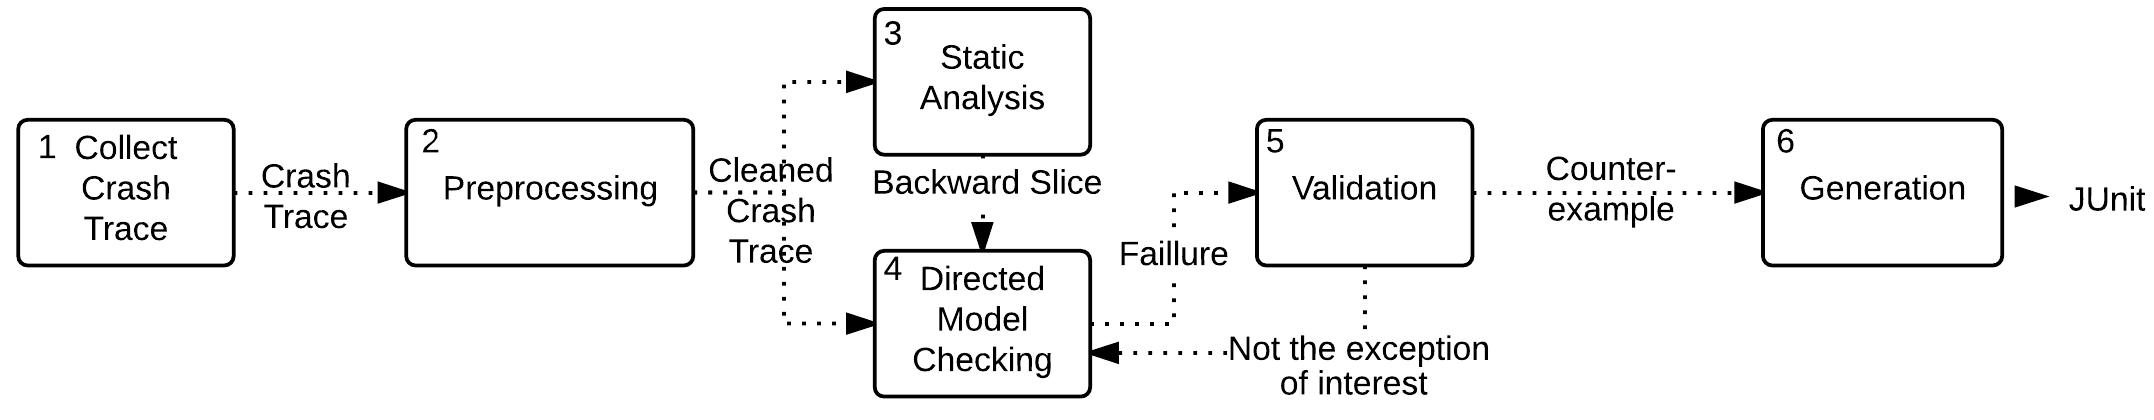
\includegraphics[scale=0.8]{media/jcharming-approach.png}
    \caption{Overview of JCHARMING.
    \label{fig:jcarming-approach}}
\end{figure}

\subsection{Collecting Crash Traces}

The first step of JCHARMING is to collect the crash trace
caused by an uncaught exception. Crash traces are usually included in crash reports and can therefore be automatically
retrieved using a simple regular expression.
Figure \ref{fig:jcarming-traces} shows an example of a crash trace that contains the
exception thrown when executing a toy-program. The crash trace contains a call to the Bar.foo()
method—the crash location point—and calls to Java standard
library functions (in this case, GUI methods because the
program was launched using a GUI).

\begin{figure}[h!]
  \noindent\fbox{%
      \parbox{\textwidth}{%
  1.javax.activity.InvalidActivityException:loopTimes \\
  should be < 3 \\
  2. at Foo.bar(Foo.java:10) \\
  3. at GUI.buttonActionPerformed(GUI.java:88) \\
  4. at GUI.access$0(GUI.java:85) \\
  5. at GUI$1.actionPerformed(GUI.java:57) \\
  6. caused by java.lang.IndexOutOfBoundsException : 3 \\
  7. at scam.Foo.buggy(Foo.java:17) \\
  8. and 4 more ...
      }%
  }
    \caption{Java InvalidActivityException is thrown in the Bar.Goo loop if the control variable is greater than 2.
    \label{fig:jcarming-traces}}
\end{figure}

As shown in Figure \ref{fig:jcarming-traces}, we can see that the first line (referred to
as frame {\it $f_0$} , subsequently the next line is called frame {\it $f_1$} , etc.)
does not represent the real crash point but it is only the last
exception of a chain of exceptions. Indeed, the {\tt InvalidActivity}
has been triggered by an {\tt IndexOutOfBoundsException} in
{\tt scam.Foo.buggy} . This kind of crash traces reflects several
nested try/catch blocks.

In addition, it is common in Java to have incomplete crash
traces. According to the Java documentation \cite{Oracle2011}, line 8 of
Figure \ref{fig:jcarming-traces} should be interpreted as follows: {\it ``This line indicates
that the remainder of the stack trace for this exception
matches the indicated number of frames from the bottom of the
stack trace of the exception that was caused by this exception
(the ``enclosing exception''). This shorthand can greatly
reduce the length of the output in the common case where a
wrapped exception is thrown from the same method as the
``causative exception'' is caught.}''

We are likely to find shortened traces in bug repositories as
they are what the user sees without any possibility to expand
their content.

\subsection{Preprocessing}

In the preprocessing step, we first reconstruct and reorganize
the crash trace in order to address the problem of nested
exceptions. Then, with the aim to obtain an optimal guidancefor our directed model checking engine, we remove frames
that are out of our control. Frames out of our controls refer
usually, but are not limited to, Java library methods and third
party libraries. In Figure \ref{fig:jcarming-traces}, we can see that Java GUI and
event management components appear in the crash trace. We
assume that these methods are not the cause of the crash;
otherwise it means that there is something wrong with the on-
field JDK. If this is the case, we will not be able to reproduce
the crash. Note that removing these unneeded frames will also
reduce the search space of the model checker.

\subsection{Building the Backward Static Slice}

For large systems, a crash trace does not necessary contain all
the methods that have been executed starting from the entry
point of the program (i.e., the main function) to the crash
location point. We need to complete the content of the crash
trace by identifying all the statements that have been executed
starting from the main function until the last line of the
preprocessed crash trace. In Figure \ref{fig:jcarming-traces}, this will be the function
call {\tt Bar.foo()}, which happens to be also the crash location
point. To achieve this, we turn to static analysis by extracting
a backward slice from the main function of the program to the
{\tt Bar.foo()} method.

A backward slice contains all possible branches that may lead
to a point {\it n} from a point {\it m} as well as the definition of the
variables that control these branches \cite{de2001program}. In other words, the
slice of a program point {\it n} is the program subset that may
influence the reachability of point {\it n} starting from point {\it m}.
The backward slice containing the branches and the definition
of the variables leading to {\it n} from {\it m} is noted as {\it $bslice_{[m \leftarrow n]}$}.

We perform a static backward slice between each frame to
compensate for possible missing information in the crash
trace. More formally, the final static backward slice is
represented as follows:

\begin{equation}
\centering
\begin{split}
bslice_{[entry \leftarrow f_0]} = bslice_{[f_1 \leftarrow f_0]} \cup bslice_{[f_2 \leftarrow f_1]} \cup ... \cup bslice_{[f_n \leftarrow f_{n−1}]} \cup bslice_{[entry \leftarrow f_n]}
\end{split}
\end{equation}

Note that the union of the slices computed between each pair
of frames must be a subset of the final slice between $f_0$ and the
entry point of the program. More formally:

\begin{equation}
\centering
\begin{split}
\bigcup_{i=0}^{entry} bslice_{[f_{i+1} \leftarrow f_i]} \subseteq bslice_{[entry \leftarrow f_0]}
\end{split}
\end{equation}

Indeed, in Figure \ref{fig:jcharming-slice}, the set of states allowing to reach $f_0$ from
$f_2$ is greater than the set of states to reach $f_1$ from $f_2$ plus set
of states to reach $f_0$ from $f_1$ . In this hypothetical example and
assuming that $z_2$ is a prerequisite to $f_2$ then
$bslice_{[entry \leftarrow f_0]} = \{f_0 , f_1 , f_2 , z_0 , z_1 , z_2 , z_3 \}$
while $\cup_{i=0}^n bslice_{[f_{i+1} \leftarrow f_i]}$.

\begin{figure}[h!]
  \centering
    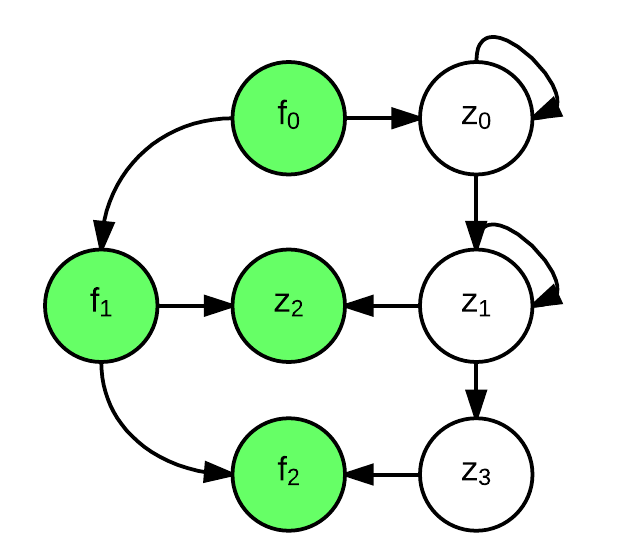
\includegraphics{media/jcharming-slices.png}
    \caption{Hypothetical example representing $bslice_{[entry \leftarrow f_0]}$ Vs. $\cup_{i=0}^n bslice_{[f_{i+1} \leftarrow f_i]} = \{f_0 , f_1 , f_2 , z_2 \}$
    \label{fig:jcharming-slice}}
\end{figure}

In the worst case scenerio where there exists one and only one
transition between each frame, which is very unlikely for real
and complex systems, then $bslice_{[entry \leftarrow f_0]}$ and
 $\cup_{i=0}^n bslice_{[f_{i+1} \leftarrow f_i]}$ yield the same set of states with a
comparable computational cost since the number of branches
to explore will be the same in both cases.

Algorithm \ref{alg:jcharming-slice} is a high level
representation of how we compute the backward slice between
each frame. The algorithm takes as input the pre-processed
call trace, the byte code of the SUT, and the entry point. From
line 1 to line 5, we initialize the different variables used by the
algorithm. The main loop of the algorithm begins at line 6 and
ends at line 15. In this loop, we compute the static slice
between the current frame and the next one. If the computed
static slice is not empty then we update the final backward
slice with the newly computed slice.


\begin{algorithm}[H]
 \KwData{Crash Stack, BCode, Entry Point}
 \KwResult{BSolve}
 $Frames~frames~\leftarrow~extract~frames~from~crash~stack$\;
 Int n $\leftarrow$ size of frame\;
 Int offset $\leftarrow$ 1\;
 Bslice bSlice $\leftarrow$ $\emptyset$\;
\For{i $\leftarrow$ 0 to i $<$ n \&\& offset $<$ n - 1}{
  BSlice currentBSlice $\leftarrow$ backward slice from frames[i] to i + offset\;
  \eIf{currentBSlice $\not=$ $\emptyset$}{
   bSlice $\leftarrow$ bSlice $\cup$ currentBSlice\;
   offset $\leftarrow$ 1\;
  }{
   offset $\leftarrow$ offset +1\;
  }
}
\caption{High level algorithm computing the union of the slices\label{alg:jcharming-slice}}
\end{algorithm}

Using backward slicing, the search space of the model checker is given by the
following expression:

\begin{equation}
  \exists x.
  \begin{pmatrix}
    \bigcup_{i=0}^{entry} bslice_{[f_{i+1} \leftarrow f_i]}  \subset SUT \\
    x.\bigcup_{i=0}^{entry} bslice_{[f_{i+1} \leftarrow f_i]}  \subset x.SUT
  \end{pmatrix}
  \models c_{i>2}
\end{equation}

That is, there exists a sequence of states transitions $x$ that
satisfies $c_{i>2}$ where both the transitions and the states are
entry
elements of $\bigcup_{i=0}^{entry} bslice_{[f_{i+1} \leftarrow f_i]}$ . Obviously, $c_{i>2}$ also
needs to be included for the final static slice to be usable by
the model checking engine. Consequently, the only frame that
need to be untouched for the backward static slice to be
meaningful is $f_0$.

\subsection{Directed Model Checking}

The model checking engine we use in this section is called JPF
(Java PathFinder) \cite{Visser2004}, which is an extensible JVM for Java
bytecode verification. This tool was first created as a front-end
for the SPIN model checker \cite{holzmann1997model} in 1999 before being open-
sourced in 2005. JPF is organized around five simple
operations: (i) {\it generate states}, (ii) {\it forward}, (iii) {\it backtrack},
(iv) {\it restore state} and (v) {\it check}. In the forward operation, the
model checking engine generates the next state $s_{t+1}$ . If
$s_{t+1}$ has successors then it is saved in a backtrack table to be
restored later. The backtrack operation consists of restoring
the last state in the backtrack table. The restore operation
allows restoring any state and can be used to restore the entire
program as it was the last time we choose between two
branches. After each, forward, backtrack and restore state
operation the check properties operation is triggered.

In order to direct JPF, we have to modify the {\it generate states}
and the {\it forward} steps. The {\it generate states} is populated with
entry
the states in $\bigcup_{i=0}^{entry} bslice_{[f_{i+1} \leftarrow f_i]}  \subset SUT$ and we adjust the
{\it forward step} to explore a state if the target state $s_i+1$ and the
transition $x$ to pass from the current state $s_i$ to $s_{i+1}$ are in
$\bigcup_{i=0}^{entry} bslice_{[f_{i+1} \leftarrow f_i]}  \subset SUT$ and $x.\bigcup_{i=0}^{entry} bslice_{[f_{i+1} \leftarrow f_i]}  \subset x.SUT$.

\subsection{Validation}

To validate the result of directed model checking, we modify
the {\it check properties} step that checks if the current sequence
of states transitions $x$ satisfies a set a property. If the current
states transitions $x$ can throw an exception, we execute $x$ and
compare the exception thrown to the original crash trace (after
preprocessing). If the two exceptions match, we conclude that
the conditions needed to trigger the failure have been met and
the bug is reproduced.

However, as argued by Kim et al. in \cite{Kim2013b}, the same failure can
be reached from different paths of the program. Although the
states executed to reach the crash are not exactly the same,
they might be useful to enhance the understanding of the bug
by software developers, and speed up the deployment of a fix.
Therefore, in this section, we consider a crash to be partially
reproduced if the crash trace generated from the model
checker matches the original crash trace by a factor of $t$, where
$t$ is a threshold specified by the user. $t$ is the percentage of
identical frames between both crash traces.

\subsection{Generating Test Cases for Bug Reproduction}

To help software developers reproduce the crash in a lab
environment we automatically produce the JUnit test cases
necessary to run the SUT to cause the exercise of the bug.

To build a test suite that reproduces a defect, we need to create
a set of objects used as arguments for the methods that will
enable us to travel from the entry point of the program to the
defect location. JPF has the ability to keep track of what
happens during model checking in the form of traces
containing the visited states and the value of the variables. We
leverage this capability to create the required objects and call
the methods leading to the failure location. Although we can
track back the internal state of objects at a specific time using
JPF, it can be too computationally taxing to recreate only the
objects needed to generate the bug. To overcome this, we use
serialization techniques \cite{Opyrchal1999}. We take advantage of features
offered by the XStream \cite{Xstream2011} library which enables the
serialization and deserialization of any Java object — even
objects that do not implement the Java Serializable interface.
We use the serialization when the model checker engine
performs too many operations modifying the property of a
given object. In such case, we serialize the last state of the
object.

\section{Case studies}

In this section, we show the effectiveness of JCHARMING to
reproduce bugs in seven open source systems\footnote{The bug reports used in this study and the result of the model checker are
made available for download from research.mathieu-
nayrolles.com/jcharming/} . The aim of the
case study is to answer the following question: {\it Can we use
crash traces and directed model checking to reproduce on-
field bugs in a reasonable amount of time?}

\subsection{Targeted Systems}

Table \ref{tab:jacharming-systems} shows the systems and their characteristics in terms of
Kilo Line of Code (KLoC) and Number of Classes (NoC).

\begin{table}[h!]
\centering
\begin{tabular}{c|c|c|c}
SUT        & KLOC & NoC  & Bug \#ID                                        \\ \hline \hline
Ant        & 265  & 1233 & 38622, 41422                                    \\
ArgoUML    & 58   & 1922 & 2603, 2558, 311, 1786                           \\
dnsjava    & 33   & 182  & 38                                              \\
jfreechart & 310  & 990  & 434, 664, 916                                   \\
Log4j      & 70   & 363  & 11570, 40212, 41186, 45335, 46271, 47912, 47957 \\
MCT        & 203  & 1267 & 440ed48                                         \\
pdfbox     & 201  & 957  & 1412, 1359 \\ \hline \hline
\end{tabular}
\caption{List of taget systems in terms of Kilo line of code (KLoC), number of classes (NoC) and Bug \# ID}
\label{tab:jacharming-systems}
\end{table}

Apache Ant \cite{ApacheSoftwareFoundation} is a popular command-line tool to build
make files. While it is mainly known for Java applications,
Apache Ant also allows building C and C++ applications. We
choose to analyze Apache Ant because it has been used by
other researchers in similar studies.

ArgoUML \cite{CollabNet} is one of the major players in the open source
UML modeling tools. It has many years of bug management
and, similar to Apache Ant, it has been extensively used as a
test subject in many studies.

Dnsjava \cite{Wellington2013} is a tool for the implementation of the DNS
mechanisms in Java. This tool can be used for queries, zone
transfers, and dynamic updates. It is not as large as the other
two, but it still makes an interesting case subject because it has
been well maintained for the past decade. Also, this tool is
used in many other popular tools such as Aspirin, Muffin and
Scarab.

JfreeChart \cite{ObjectRefineryLimited2005} is a well-known library that enables the
creation of professional charts. Similar to dnsjava, it has been
maintained over a very long period of time —JfreeChart was
created in 2005— and it is a relatively large application.

Apache Log4j \cite{TheApacheSoftwareFoundation1999} is a logging library for Java. This is not a
very large library, but it is extensively used by thousands of
programs. As other Apache projects, this tool is well
maintained by a strong open source community and allows
developers to submit bugs. The bugs which are in the bug
report system of Log4j are, generally speaking, well
documented and almost every bug contains a related crash
trace and, therefore, it is a tool of interest to us.

MCT \cite{NASA2009} stands for Mission Control technologies and was
developed by the NASA Ames Research Center (the creators
of JPF) for use in spaceflight mission operation. This tool
benefits from two years of history and targets a very critical
domain, Spacial Mission Control. Therefore, this tool has to
be particularly and carefully tested and, consequently, the
remaining bugs should be hard to discover and reproduce.

PDFBox \cite{ApacheSoftwareFoundation2014} is another tool supported by the Apache
Software Foundation since 2009 and was created in 2008.
PDFBox allows the creation of new PDF documents and the
manipulation of existing documents.

\subsection{Bug Selection and Crash Traces}

In this study, we have selected the reproduced bugs randomly
in order to avoid the introduction of any bias. We selected a
random number of bugs ranging from 1 to 10 for each SUT
containing the word ``exception'' and where the description of
the bug contains a match a regular expression designed to find the pattern of a
Java exception.

\section{Results}

Table \ref{tab:jcharming-results} shows the results of JCHARMING in terms of Bug
\#ID, reproduction status, and execution time (in minutes) of
directed model checking (DMC) and Model Checking (MC).
The experiments have been conducted on a Linux machine (8
GB of RAM and using Java 1.7.0\_51).

\begin{itemize}
  \item The result is noted as ``Yes'' if the bug has been fully
reproduced, meaning that the crash trace generated by the
model checker is identical to the crash trace collected
during the failure of the system.
\item The result is ``Partial'' if the similarity between the crash
trace generated by the model checker and the original
crash trace is above t=80\%. Given an 80\% similarity
threshold, we consider partial reproduction as successful.
A different threshold could be used.
\item Finally, the result of the approach is reported as ``No'' if
either the similarity is below t < 80\% or the model
checker failed to crash the system given the input we
provided.
\end{itemize}

\begin{table}[h!]
\centering
\begin{tabular}{c|c|c|c|c}
SUT                         & Bug \#ID & Reprod. & Time DMC & Time MC \\ \hline \hline
\multirow{2}{*}{Ant}        & 38622    & Yes     & 25.4     & -       \\
                            & 41422    & No      & -        & -       \\ \hline
\multirow{4}{*}{ArgoUML}    & 2558     & Partial & 10.6     & -       \\
                            & 2603     & Partial & 9.4      & -       \\
                            & 311      & Yes     & 11.3     & -       \\
                            & 1786     & Partial & 9.9      & -       \\  \hline
DnsJava                     & 38       & Yes     & 4        & 23      \\ \hline
\multirow{3}{*}{jFreeChart} & 434      & Yes     & 27.3     & -       \\
                            & 664      & Partial & 31.2     & -       \\
                            & 916      & Yes     & 26.4     & -       \\ \hline
\multirow{7}{*}{Log4j}      & 11570    & Yes     & 12.1     & -       \\
                            & 40212    & Yes     & 15.8     & -       \\
                            & 41186    & Partial & 16.7     & -       \\
                            & 45335    & No      & -        & -       \\
                            & 46271    & Yes     & 13.9    & -       \\
                            & 47912    & Yes     & 12.3     & -       \\
                            & 47957    & No      & -        & -       \\
MCT                         & 440ed48  & Yes     & 18.6     & -       \\ \hline
\multirow{2}{*}{PDFBox}     & 1412     & Partial & 19.7     & -       \\
                            & 1359     & No      & -        & - \\ \hline \hline
\end{tabular}

\caption{Effectiveness of JCHARMING using directed model checking (DMC) and model checking (MC) in minutes}
\label{tab:jcharming-results}
\end{table}

As we can see in Table \ref{tab:jcharming-results}, we were able to reproduce 17 bugs
out of 20 bugs either completely or partially (85% success
ratio). The average time to reproduce a bug is 16 minutes.
This result demonstrates the effectiveness of our approach,
more particularly, the use of backward slicing to create a
manageable search space that guides adequately the model
checking engine. We also believe that our approach is usable
in practice since it is also time efficient.
